\documentclass[12pt]{article}
\usepackage{parskip}
\usepackage{amsmath}
\usepackage{pdfpages}
\usepackage{listings}
\usepackage{color}
\usepackage[margin=.6in]{geometry}

\definecolor{dkgreen}{rgb}{0,0.6,0}
\definecolor{gray}{rgb}{0.5,0.5,0.5}
\definecolor{mauve}{rgb}{0.58,0,0.82}

\lstset{frame=tb,
  language=C++,
  aboveskip=3mm,
  belowskip=3mm,
  showstringspaces=false,
  columns=flexible,
  basicstyle={\small\ttfamily},
  numbers=none,
  numberstyle=\tiny\color{gray},
  keywordstyle=\color{blue},
  commentstyle=\color{dkgreen},
  stringstyle=\color{mauve},
  breaklines=true,
  breakatwhitespace=true,
  tabsize=3
}
\
\begin{document}
\includepdf[pages=2-3]{slides.pdf}
Usually the ethernet exists as hub that all other devices are connected. Any packet that gets put on the bus just gets sent to every port on the bus.

\includepdf[pages=4]{slides.pdf}
CSMA/CD is carrier sense multiple access collision detection. This means that before you submit a packet to the bus you check if the carrier has traffic on it. When you send a packet you can only send it one bit at a time which can be problematic as someone else can start submitting while you are still sending. This is called \textbf{trasmission delay}. Another problem that occurs is that it takes time for the bit to actually move down the wire which can cause a collision. This is called \textbf{propogation delay}.

\includepdf[pages=5-6]{slides.pdf}
A collision is just when there is more than one bit moving on the bus. We can calculate the propagation delay and the size of our packet and such to know which fame caused a collision. If its ours we can resend the packet to try again. These retransmission attempts will occur 16 times (this is just a magic number). We delay by a random amount of time (chose number and multiply by the time it takes to traverse). 

\includepdf[pages=7]{slides.pdf}
The performance of shared ethernet is god awful. This resulted in the invention of switched internet. For this the packet on the ethernet only gets sent to the port that it actually wants to. When it first gets turned on it behaves like a hub, but as packets are sent it builds a table of addresses for the various devices on the network. When a device sends something it notes its address.

\includepdf[pages=8]{slides.pdf}
Over the years switches got hella powerful with tons of ports. You can extend your network using vlan. When the switch is building its table of devices it also records a vlan id for each one. If a device tries to send a packet to a device of a different vlan id the switch will not send it. This allows us to segregate our network. 

\includepdf[pages=9-10]{slides.pdf}
If you still want to send a packet to a different vlan you can do it by sending it through a higher level of protocol (like sending it through ip). You could also bridge the two devices. Basically making a special entry saying that its totally ok for those two to talk in the switch's table.

\includepdf[pages=11]{slides.pdf}
\includepdf[pages=14]{slides.pdf}
We can create connections between devices, by physically wiring them together, ignoring the switch. This makes it easier to talk since they don't have to make as many hops. We also have redundancy if someone where to remove one of those wires. On the flipside we can run into problems with loops. The devices don't have switching tables, so they have to build them. When a devices gets a packet it sends to out on all of its ports (it doesnt have a switch table built up yet). As the packet hits those devices they do the same thing which makes A update its switch table. 

\includepdf[pages=15]{slides.pdf}
This causes a shit ton of packets to get sent out. Because those packets are getting sent everywhere the switch tables stored on devices oscillate like crazy.

\includepdf[pages=16]{slides.pdf}
The solution to this is to build a spanning tree out of all of your connected devices. A super efficient way to do this is through a simple breadth first search. If you have weights and care about it you can use Prim's algorithm.

\includepdf[pages=17-18]{slides.pdf}
\includepdf[pages=19-21]{slides.pdf}
When we build the spanning three we send out a bunch of special packets that the switches know contain nothing and handle properly. With this we build a rooted tree. As we build we record numbers on the devices so that we can tell that the device with the smallest number is the root relative to you. Before it has received a packet all devices think they are the root. As packets go through they re-evaluate this based on the packet age. Devices create designated root ports and designated designated ports through which its children can send to the root through it. It takes about a minute of it building its shit when you reboot your ethernet switch.

\includepdf[pages=22]{slides.pdf}

\includepdf[pages=23]{slides.pdf}
Even in point to point connections shit can get complicated. We send a bunch of configuration and authentication requests with a bunch of acknowledgements and responses. In this image you can see all the crap bouncing back and forth for a simple device to device connection.
Stevens
\includepdf[pages=24-25]{slides.pdf}
ARP is how we resolve conflicting addresses. We have a special box that checks for any matching addresses. If there aren't any the ARP box gives the go-ahead and the ethernet driver can construct the ethernet frame and send its shit out.

ARP works by building a dummy frame. It includes ethernet information (destination, source, and type). Then you have the ARP frame. It contains the sender and target's hardware address (the ethernet address) and protocol address(the ipaddress). The sender just fills that in with its own information. If you are send it locally, you know that the target's protocol address is the same as yourse (since it is on the same network). Problem is, you don't know the target's hardware address. This is why we have a request or response value stored in the op field. In a request the target hardware address is all 0s since you dont know it. If you don't know the destination address you can fill in all 1s which the protocol knows that its a broadcast frame, so the device that it hits just absorbs it. It then populates the target hardware address and sends a response. This will be unicast (the destination address is the device we are looking at).

We \textbf{resolve} addresses, not translate the.







\end{document}